\section{Projekt}

Zgodnie z dokumentacją RXHDR\_V2 \cite{master} na szesnastu wyjściach cyfrowych uzyskiwany jest sygnał o logice 0 do 1.8V o czasie trwania między 50ns a 200ns i częstotliwości osiągającej nawet do 2.5 MHz.
Sygnał ten na potrzeby rozwiązań softwarowych jest modyfikowany przez translator poziomów do poziomów logicznych 0 - 3.6V i zostaje wybierana ósemka z szesnastu kanałów przez dyskryminator.   
Tak wybrane ósemki mają nazwę 1A0-7 dla pierwszej oraz 2A0-7 dla drugiej części wyjść.   
Otrzymane sygnały należy zliczyć na płytce Arduino Due w ściśle określonym czasie oraz przekazać dane do dalszej obróbki bądź wizualizacji na zewnętrznym komputerze.

Cały proces kompilacji kodu C++ do kodu Asemblera został wykonany na kompilatorze ARM gcc 4.6.4 (linux). 

W poniższych rozdziałach opisane są proponowane sposoby wykonania tego zadania. 

\subsection{Rozwiązanie softwarowe na platformie Arduino}
\label{dzial arduino}
Założeniem rozwiązania jest bezpośrednie zliczenie sygnałów z wykorzystaniem przerwań sprzętowych w frameworku Arduino. W tym celu stosowane są wyjścia cyfrowe płytki Arduino due oraz dyskriminatora sygnałów zmniejszającego liczbę wyjść płytki z 16 do 8.
Zbocze każdego z tak dyskryminowanego sygnału  powoduje wywołanie krótkiej dedykowanej funkcji zwiększającej wartość licznika o jeden. 

Fragment kodu \ref{code_ard_IRS} jest częścią programu użytego do badań. Na potrzeby badania zostaje uwzględniony tylko pojedynczy kanał.

\begin{kod}
        \lstinputlisting[language=C++, firstline=95, lastline=117]{code_source/arduino/monocanal_rst.cpp}
        \caption{Fragment kodu użytego do testowania rozwiązania z przerwaniami systemowymi.}
        \label{code_ard_IRS}
\end{kod}


Używana płytka rozwojowa Arduino Due, używa mikrokontrolera AT91SAM3X8E w architekturze 32 bitowej o taktowaniu głównego procesora równemu 84 MHz.

Pomimo krótkiej operacji wewnątrz IRS (eng. interupt service rutine) - \textit{add} (tabela \ref{decompile add}) proces wejścia do rutyny przerwania i wyjścia zabiera nieporównywalnie więcej cykli procesora, co powoduje że cały proces wywołania przerwania jest kosztowny w czasie. 
Ilość cykli procesora koniecznych do wywołania funkcji przerwania używając nieoptymalizowanego kodu Arduino może wymagać nawet do 355 cykli procesora \cite{ard_opt_git}, dodatkowo powrót do głównego wątku programu może wymagać kolejnych 128 cykli \cite{ard_opt_git}.

\begin{table}{h}
        \begin{center}
        \caption{Estymacja ilości cyklów procesora koniecznych do wykonania instrukcji umieszczonych w funkcji \textit{add} }
        \label{decompile add}
        \begin{tabular}{c|c|c}
                kod C++ & pseudo kod Asemblera & Ilość cykli procesora \cite{cycles} \\ \hline
                val++ & LDR & 1-2 \\
                        & ADD & 1 \\
                        & STR & 1-2 \\ 
                        \hline \hline
                        &   &  3-5 
        \end{tabular}
        \end{center}
\end{table}

Pojedynczy cykl procesora zgodnie z wzorem \ref{Cykli w sec} dla układu Arduino Due trwa ~$ 11.9 ns $. 
Oznacza to że wykonanie instrukcji \textit{val ++} zgodnie z najgorszą estymacja (tabela \ref{decompile add}) trwa ~ $59.52 ns$. 
Jednak po dodaniu czasu koniecznego na wywołanie i powrót z IRS otrzymywany jest czas $ (355 + 128 + 5) * 11.9 ns =  5.8072 \mu s $. 

Podczas wywołania przerwania o tym samym priorytecie co priorytet tego właśnie wykonywanego, sygnał wywołujący zostanie zapamiętany i ewaluowany zaraz po wyjściu z właśnie wykonywanego IRS  \cite{datasheet}. 
Oznacza to że w przypadku generowania sygnałów o większej częstotliwości niż jest możliwa ich ewaluacja, doprowadzamy do sytuacji kiedy nigdy nie wrócimy do normalnego przebiegu programu. 

Zgodnie z wymaganiami projektu uzyskiwane sygnały wymagające zliczenia mogą przychodzić z częstotliwością nawet do $2.5MHz$ co oznacza kolejny sygnał przychodzący co $0.4\mu s$.
Takie wymagania oznaczają że już dla pojedynczego kanału takie rozwiązanie jest niewystarczające. 

\subsection{Rozwiązanie softwarowe w standardzie CMSIS}
Główną filozofią platformy Arduiono jest możliwość przenoszenia kodu między różnymi urządzeniami należącymi do dużej rodziny Arduino oraz łatwość programowania.
W celu osiągnięcia tych dwóch celów często poświęcana jest szybkość działania. 

Dodatkowo platforma Arduino implementuje funkcję których działanie może wpływać na pracę mikrokontrolera nawet bez ich wywoływania. 
Przykładowo na potrzeby działania funkcji \textit{milis()} konieczna jest specyficzna konfiguracja głównego zegara i cykliczne wywoływanie przerwań w celu implementacji licznika. Powoduje to kolejne spowolnienia działania programów. 


CMSIS to biblioteka udostępniająca warstwę abstrakcji dla mikrokontrolerów używających procesorów grupy ARM Cortex. 
Pozwala ona na niskopoziomowe programowanie procesorów tego typu ze skupieniem na szybkości działania.

Zgodnie z notą producenta \cite{interupt latency} w najbardziej optymalnej sytuacji dla procesora \textit{Cortex-M3} wejście do funkcji przerwania sprzętowego wymaga 12 cykli, a wyjście można osiągnąć w 10 cyklach. 
Przy tak optymistycznej estymacji możliwe byłoby osiągnięcie częstotliwości zliczeń nawet do $\frac{1}{11.9ns*27} = ~ 3.11 MHz$, jednak ponieważ zliczenia z różnych kanałów nie mogą być ewaluowane równolegle wynik ten nadal jest niewystarczający. 

Dodatkowo bez dostępu do debugera rozwiązywanie problemów pojawiających się podczas programowania w tym podejściu okazały się niewarte włożonej pracy. 

Z tych dwóch powodów rozwiązanie to zostało porzucone i nie wykonano badań w takim układzie. 

\subsection{Rozwiązanie z użyciem dodatkowego układu elektronicznego.}

Wykorzystanie rozwiązania z dodatkowym układem elektroniki przy wykorzystaniu frameworku Arduino. Celem dodatkowego elementu elektronicznego jest ułatwienie odczytu zliczeń przez mikrokontroler oraz zmniejszenie wymaganej częstotliwości zliczeń. 

\subsubsection{Układ liczników zewnętrznych}
\label{section licziki}

W celu rozwiązania problemu wysokiej częstotliwości zliczeń otrzymywanych z układu RXHDR\_V2 \cite{master} zastosowano zestaw ośmiu binarnych liczników 4-bitowych \cite{licznik doc}. 


\begin{figure}[]
        \centering
        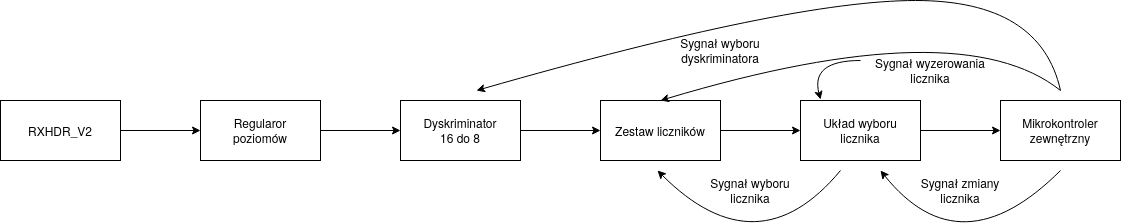
\includegraphics[width=\textwidth]{Elektronika_flow_chart.png}
        \caption{Schemat działania układu liczników zewnętrznych i sygnałów kontrolujących}
        \label{licznik flowchart}
\end{figure}

Schemat ideowy układu znajduje się na obrazku \ref{licznik flowchart}.
Na tym schemacie znajdują się sygnały kontrolujące pracę układu. Poniżej zdefiniowane jest nazewnictwo sygnałów na schematach elektronicznych i ich funkcja.  
\begin{itemize}
        \item ReadCLC - Sygnał zmiany licznika - pojedynczej przejście stanu z niskiego na wyskoki powoduje wybór kolejnego licznika do odczytu
        \item RC\_B - Sygnał wyzerowania licznika - stan niski powoduje wyzerowanie liczników i ustawienie układów do stanu początkowego.
        \item DIS\_S - Sygnał wyboru dyskryminatora - Stan niski powoduje wybranie sygnałów 1A0-7 a wysoki 2A0-7
        \item ENP0-7 - Sygnał wyboru licznika - osiem osobnych linii których stan niski pozwala na wybór licznika do odczytu. Podczas odczytu tylko jeden z sygnałów powinien być w stanie niskim reszta powinna utrzymywać stan wysoki. 
\end{itemize}
Sygnał otrzymywany przez układ RXHDR\_V2 jest przepuszczany przez translator poziomów w celu zmiany logiki z 0-1.8$V$ do 0-3.6$V$. Następnie z 16 kanałów zostaje wybrane 8, tak opracowane sygnały trafiają na układ liczników.

\paragraph{Układ liczników \cite{licznik doc}\cite{slave}}

4-bitowy binarny licznik SN74LV161A ma 9 wejść logicznych. 
W tym układzie licznik znajduje się w następującej konfiguracji:
\begin{itemize}
        \item $CLC$ - Tu podawany jest sygnał zliczeń i on jest zliczany aż do przepełnienia licznika.
        \item $\overline{CLR}$ - Połączone z linią RC\_B, stan niski powoduje wstrzymanie pracy i wyzerowanie wartości przechowywanych w liczniku. 
        \item $ENT,ENP$ - w celu stabilizacji układu na czas odczytywania wartości chcemy wstrzymać zliczanie dlatego też ustalamy stan wysoki dla wejścia ENT i wejście ENP łączymy z kanałem ENP0-7 odpowiadającym odpowiedniemu licznikowi.
        Sprawia to że wraz z wyborem licznika układ ustala swój stan i nie zmienia go aż do chwili wyboru następnego. 
        Jest to sposób na uniknięcie niepewności i błędów wynikających z odczytywania zmieniającej się wartości, jednak powoduje to powstanie czasu martwego w układzie podczas którego wartości nie będą zliczane na odczytywanym liczniku.
        \item $A,B,C,D$ - funkcja ładowania wartości nie jest używana wejścia te są uziemione
        \item $\overline{LOAD}$ - funkcja ładowania wartości nie jest używana wejście to jest uziemione
\end{itemize} 

Na wyjściu wykorzystane są jedynie linie Q0-3 to one podają binarnie przechowywaną wartość. 
Tak skonfigurowane liczniki będą zliczać wartości otrzymywane przez wejście $CLC$ aż do osiągnięcia wartości 16 kiedy to licznik zostaje przepełniony i podawana przez niego wartość wraca do 0. 

\paragraph{Układ wyboru sygnału}

Celem tego układu jest zmiana sygnału zmiany licznika na sygnał wyboru licznika. W tym celu wykorzystany jest rejestr przesuwany. 
Wybrany układ służący temu zadaniu to SN74LV164A\cite{shift doc}, jest on szeregowo-równoległym rejestrem co oznacza ze dane wejściowe są dostarczane szeregowo a otrzymywana jest informacja równoległa która jest przesuwana wraz z kolejnymi sygnałami zegara. Dokumentacja rejestru SN74LV164A mówi o dwóch wejściach jednak są one bezpośrednio wyprowadzane na bramkę logiczną AND co sprawia że układ ten spełnia warunek pojedynczego wejścia rejestru szeregowo-równoległego. W konfiguracji tego układu gdzie oba wejścia są ze sobą zwarte, bramka logiczna AND jest ignorowana.
Schemat układu wyboru licznika znajduje się rysunku \ref{wybor schema}. 

\begin{figure}
        \begin{multicols}{2}
                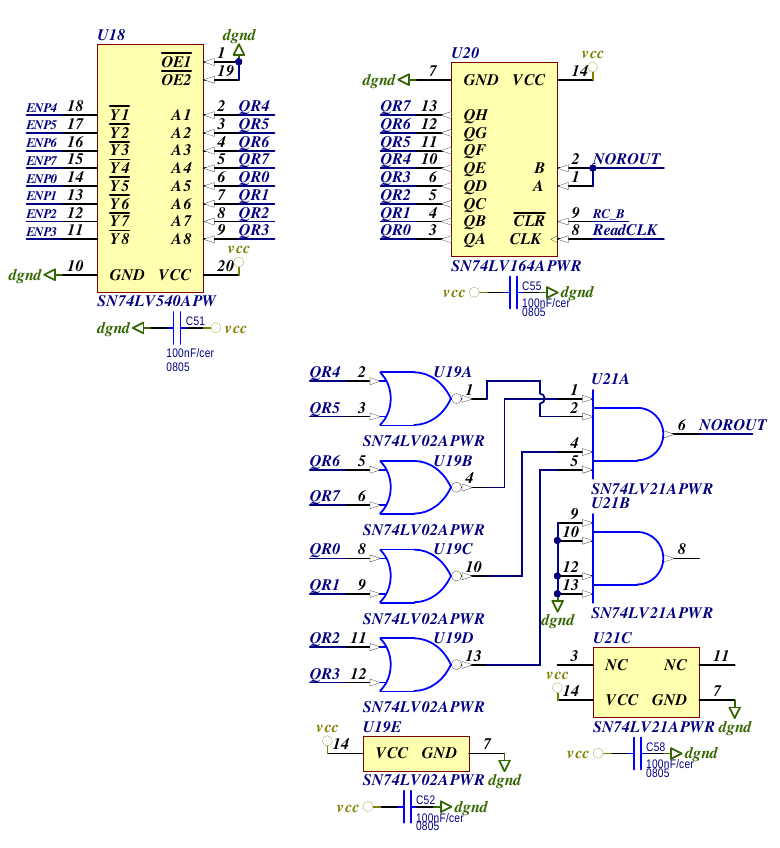
\includegraphics[width=0.45\textwidth]{shift_register.png}
                \caption{Schemat układu wyboru licznika wykorzystujący rejestr przesuwny.}
                \label{wybor schema}
                \par
                \hfill
                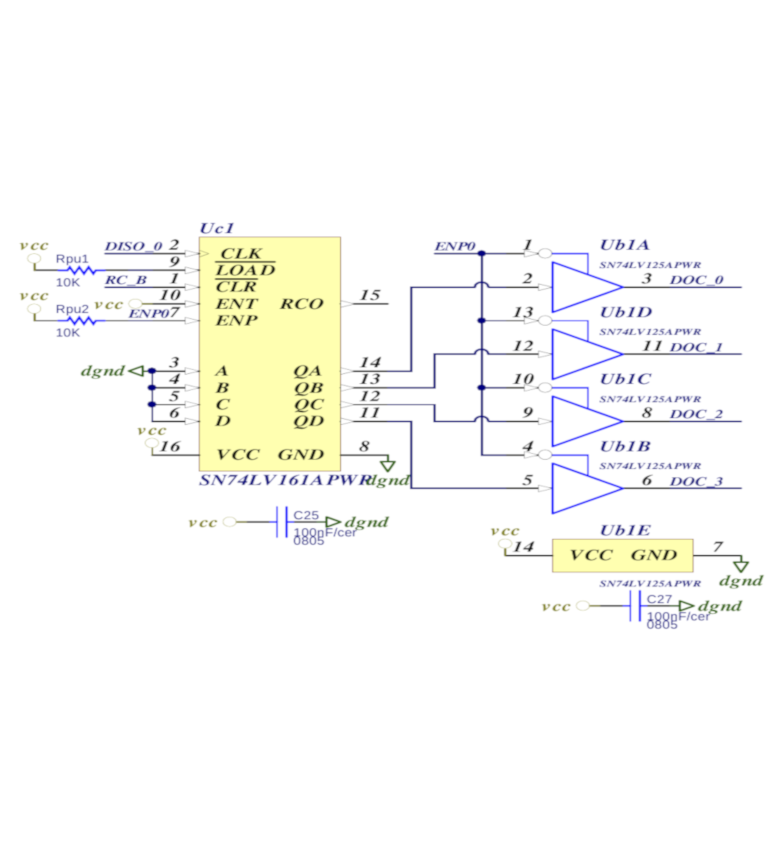
\includegraphics[width=0.45\textwidth]{Licznik.png}
                \caption{Schemat konfiguracji jednego z używanych liczników wraz z częścią multipleksera wyjściowego.}
                \label{licznik}
                \par
                \hfill
        \end{multicols} 
\end{figure}

W celu osiągnięcia efektu pojedynczej wartości logicznej która przesuwa się z każdym rosnącym zboczem sygnału na wejściu rejestru musimy dostarczyć pojedynczy niski, stan podczas pierwszego cyklu pracy, a następnie trzymać stan wysoki aż do chwili potrzeby powtórzenia cyklu. 
Za pomocą bramek NOR układu SN74LV02A oraz bramek AND układu SN74LV21A osiągamy równanie logiczne:
\begin{equation}
        NOROUT = \overline{(QR1*QR2)} + \overline{(QR3*QR4)} + \overline{(QR5*QR6)} + \overline{(QR7*QR8)}
\end{equation}
Gdzie:
\begin{itemize}
        \item $NOROUT$ - Sygnał wejściowy rejestru 
        \item $QR1-8$ - Wyjścia rejestru. 
\end{itemize}

\begin{table}
        \centering
        \caption{Cykl działania rejestru przesuwnego układu wyboru licznika}
        \label{shift sygnal}
        \begin{tabular}{lccccccccc}
                Czas &$QR1$&$QR2$&$QR3$&$QR4$&$QR5$&$QR6$&$QR7$&$QR8$  &NOROUT\\ \hline     
                T1&H&H&H&H&H&H&H&H &L\\
                T2&L&H&H&H&H&H&H&H &H\\
                T3&H&L&H&H&H&H&H&H &H\\
                T4&H&H&L&H&H&H&H&H &H\\
                T5&H&H&H&L&H&H&H&H &H\\
                T6&H&H&H&H&L&H&H&H &H\\
                T7&H&H&H&H&H&L&H&H &H\\
                T8&H&H&H&H&H&H&L&H &H\\
                T9&H&H&H&H&H&H&H&L &H\\
                T10&H&H&H&H&H&H&H&H &L\\
        \end{tabular}
\end{table}

Sekwencja sygnału pokazana jest w tabeli \ref{shift sygnal}. Na tej wizualizacji widać że gdyby w konfiguracji zastąpić linię $QR8$ połączeniem do zasilania możliwe byłoby ograniczenie liczby sekwencji w cyklu do 8. Jednak dzięki tej pojedynczej sekwencji gdy żaden z liczników nie jest odczytywany otrzymujemy cykl podczas którego żaden z liczników nie jest zablokowany i wszystkie kontynuują liczenie. 

W ten sposób otrzymywany sygnał następnie jest negowany przez układ SN74LV540 i dostarczany do multipleksera pokazanego na rysunku \ref{licznik}.
Tu zestaw wzmacniaczy operacyjnych sprawia ze tylko tylko licznik dla odpowiadającego sygnału ENP o niskim stanie ustala stan na zewnętrznych wyjściach. 

\paragraph{Czas martwy i szybkość odczytu układu licznika}

\begin{figure}
        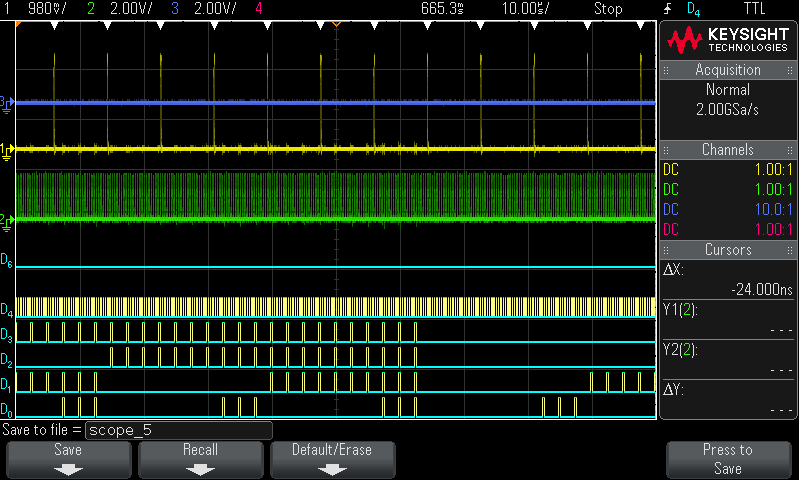
\includegraphics[width=\textwidth]{scope_1.png}
        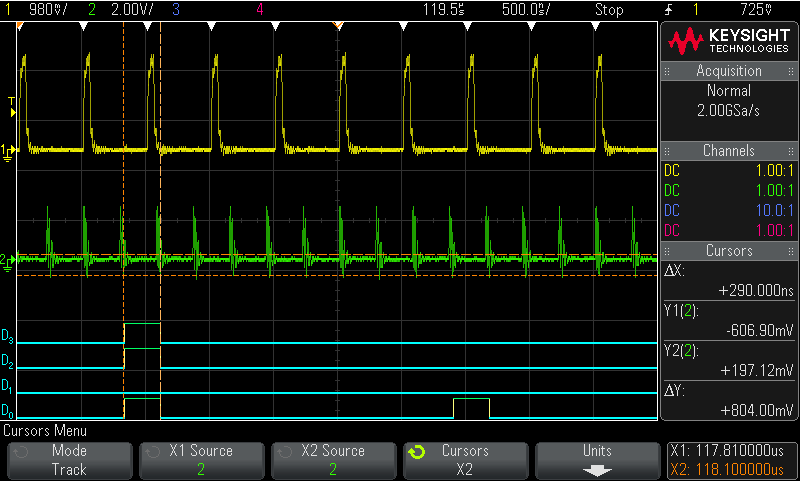
\includegraphics[width=\textwidth]{scope_2.png}
        \caption{Rzuty ekranu z oscyloskopu podłączonego do płytki. 
        Impulsy wejściowe (żółte) są wprowadzane na jeden z kanałów. 
        Sygnał D0-3 pokazuje binarne zliczanie na danym kanale. 
        Na górnym zrzucie widać że w przypadku nie zarejestrowania następnego sygnału wyjście dla kanału się powtarza. 
        Na dolnym obrazku widoczny jest impuls trafiający na czas martwy będący chwilą odczytu wartości z kanału.
        Następuje przeskok z wartości $1101_{2}$ ($13_{10}$) na $0001_{2}$ ($1_{10}$) mimo faktu że wystąpiło 5 impulsów.
        }
        \label{Oscyloskop}
\end{figure}

Podczas odczytu licznika informacja o zliczeniach zostaje tracona oznacza to że układ ten generuje czas martwy. 
Procentowa długość tego czasu może być wyznaczona na podstawie wzoru:
\begin{equation}
        T_d = \frac{T_o/N_l}{T_o+T_e} * 100\%
\end{equation}
Gdzie:
\begin{itemize}
        \item $T_d$ - procentowy czas martwy licznika.
        \item $T_o$ - czas odczytu.
        \item $N_l$ - liczba liczników w sekwencji odczytu. W używanej konfiguracji jest to osiem liczników. 
        \item $T_e$ - czas pustego cyklu.
\end{itemize}

Oznacza to że przedłużając czas pustego cyklu zmniejszamy czas martwy układu, jednak ponieważ liczniki mogą jedynie 16 stanów to konieczne jest odczytanie ich przed zliczeniem 16 liczby. 
Oznacza to że:
\begin{equation}
        T_o+T_e * F \leqslant 15
\end{equation}
        Gdzie:
\begin{itemize}
        \item $F$ - spodziewana częstotliwość zliczeń
\end{itemize}

Dla podanych wymagań: 2.5 miliona zliczeń na sekundę, można wyliczyć że suma czasu odczytu i pustych sekwencji powinna być mniejsza niż 6$\mu s$.
Oznacza to że sekwencja odczytu powinna zmieścić się w 504 cyklach procesora. 

\subsubsection{Oprogramowanie mikrokontrolera}

Zadaniem mikrokontrolera jest odebranie danych z układu wspomagającego w czasie uniemożliwiającym przepełnienie liczników i wysłanie sformatowanych danych na komputer zewnętrzy. 

\paragraph{Wymagane połączenie}
W celu utworzenia funkcjonującego układu akwizycji zliczeń konieczne jest połączenie kablem USB2.0 typ A/micro-USB typ B między komputerem sterującym a natywnym portem Arduino Due (Port bliżej przycisku resetu).

Dodatkowo wymagane jest połączenie z płytką zewnętrzną. Konieczne połączenia to:
\begin{itemize}
        \item Połączenia $DOC\_0-4\_ext$ w domyślnej konfiguracji powinny być połączone z wyjściami arduino o pinach 33-36 - są to wyjścia liczników.
        \item $ReadCLC$ - arduino pin 25 - wyjście sygnału zmiany licznika
        \item $RC\_B\_ext$ - arduino pin 26 - wyjście sygnału resetu liczników 
        \item $DIS\_S\_ext$ - arduino pin 27 - wyjście sygnału wyboru dyskryminatora
        \item Dodatkowo koniecznie jest ustalenie wspólnego uziemienia w celu stabilizacji poziomów logicznych.
\end{itemize}

Są to wyjścia w domyślnej konfiguracji i można dokonać zmiany poprzez modyfikację pliku \textit{USER\_CONFIG.h}.



\paragraph{Akwizycja danych}
Dane otrzymywane z zewnętrznego układu elektronicznego (dział \ref{section licziki}) mają postać binarnej liczby 4-pozycyjnej rosnącej do wartości 15 a następnie zawijające się ponownie do liczby 0. 
Dzięki tej formie prezentacji danych po odczytaniu stanów logicznych na urządzeniu peryferyjnym i odpowiednim przesunięciu logicznym w prosty sposób otrzymujemy wartość na liczniku. 
Podejście to jednak wymaga specyficznego połączenia oraz uwzględnienia potencjalnego przepełnienia licznika. 

W jednym cyklu akwizycji zostaje wybierany pierwsze osiem liczników 1A0-7 następnie przez czas akwizycji, korygowanej o czas martwy, zbierane są dane z liczników i dodawane do miejsca w tablicy odpowiadającemu odpowiedniemu licznikowi, następnie zmieniana jest ósemka badanych liczników i proces ponownie jest powtarzany. 

Proces akwizycji danych musi być bardzo dokładnie kontrolowany pod względem czasu wykonania.
Czas pobierania danych jest regulowany przez ilość pętli Podczas których dokonywana jest akwizycja danych. 
Przykład tej pętli znajduje się w fragmencie kodu \ref{code aqw}.

\begin{kod}
        \lstinputlisting[language=C++, firstline=76, lastline=103]{code_source/arduino/final.cpp}
        \caption{Fragment kodu odpowiedzialnego za akwizycję danych}
        \label{code aqw}
\end{kod}

Jak widać ilość iteracji jest ustalana przez wymagany czas w milisekundach po korekcjach o czas martwy licznika oraz z uwzględnieniem ilości czasu przypadającego na pojedynczą pętlę. 
Warunkiem koniecznym takiego podejścia jest stały czas wykonywania iteracji pętli. 
Różnice w czasie mogą być powodowane przez operacje dostępu do pamięci kiedy to w różnych iteracjach stosujemy dostęp do pamięci a w innych wykorzystujemy wcześniej przygotowane rejestry.
Drugim powodem mogą być rozwidlenia pracy programu, sytuacje kiedy przebieg programu jest uwarunkowany wynikiem jakiegoś warunku i dwie drogi potrzebują różną ilość cykli procesora na wykonanie. 
W celu analizy takich sytuacji przydatna jest analiza skompilowanego kodu c do kodu asemblera.
Fragment krytycznej części programu jest przedstawiony w wycinku kodu \ref{asembly}.

\begin{kod}
        \lstinputlisting[language={[Motorola68k]Assembler},firstline=30, lastline=48]{code_source/asembler/loop_final.S}
        \caption{Fragment kodu asemblera utworzonego przez kompilację części kodu \ref{code aqw}. }
        \label{asembly}
\end{kod}

Po analizie kodu \ref{asembly} można stwierdzić że nie zdarza się sytuacja żeby w różnych iteracjach występowała różna ilość dostępów do pamięci.
Jak jednak widać w fragmencie programu \ref{code aqw} w przypadku wystąpienia przepełnienia licznika konieczne jest dodanie wartości pełnego licznika do otrzymanej liczby. 
Powoduje to że wymagana jest dodatkowa instrukcja add.

Jednak proces warunkowego dodania jest realizowany przez specyficzną instrukcję it.
Należy ona do zestawu instrukcji Thumb®-2 i pozwala na uniknięcie problemów wynikających z warunkowej zmiany biegu programu dla krótkich instrukcji. 
Zgodnie z dokumentacją\cite{cycles} cortex-M3 czas potrzebny na wykonanie tej instrukcji to jeden cykl procesora, jednak jest sprecyzowane że instrukcja może być dołączona do następnej instrukcji pozwalając na wykonanie w tym samym czasie co następna komenda.
Tak się dzieje w przypadku spełnienia warunku gt (eng. greater then - większy niż) poprzedniej instrukcji cmp. Jednak jeżeli warunek ten nie zostaje spełniony to ewaluacja instrukcji it zwiększa się do jednego cyklu i przechodzi do warunku else (druga instrukcja w kolejności).
Cały ten proces sprawia że tak samo w przypadku spełniania warunku gt jak i w przypadku niezgodności ten fragment kodu wymaga dwóch cykli procesora.
$$it(1c) + rsb(1c) = it(0c) + add(1c) + rsb(1c)$$

\paragraph{Komunikacja z komputerem zewnętrznym}
Ze względu na fakt że proces akwizycji danych jest tak wrażliwy na wszelkie zmiany ilości poleceń konieczne jest wyłączenie obsługi przerwań w trakcie wykonywania kluczowego fragment programu. 
Sprawia to że w trakcie akwizycji obsługa komunikacji z zewnętrznymi urządzeniami przez układy komunikacji seryjnej jest niemożliwa. 
Oznacza to że wymagana jest bardzo dokładna obsługa komunikacji z zwróceniem szczególnej uwagi na potencjalne błędy. 

W tabeli \ref{komunikacja} znajdują się komendy i odpowiedzi stosowane w komunikacji między urządzeniami. 
Forma wszelkich stałych komunikacyjnych znajduje się w osobnym pliku \textit{USER\_CONFIG.h} pozwalającym na łatwą zmianę prezentowanych komend.

\begin{table}
        \centering
        \caption{Tabela komend stosowanych w celu komunikacji między komputerem zewnętrznym a mikrokontrolerem}
        \label{komunikacja}
        \begin{tabularx}{\textwidth}{|c|c|X|}
                \hline
                komenda & odpowiedź & opis \\ \hline

                \textbackslash n & Ready to read\textbackslash n & 
                Krótki znak rozpoczynający komunikację.
                Po otrzymaniu tego symbolu mikrokontroler wstrzymuje proces akwizycji i oczekuje na dalsze polecenia.
                Przed wysłaniem dowolnej komendy konieczne jest poprzedzenie tym symbolem, w celu upewnienia się że mikrokontroler jest gotowy na zmianę trybu pracy.
                \\ \hline

                42a\textbackslash n & 42b\textbackslash n& Krótka komenda, nie zmieniająca nic w pracy licznika. Pozwala na sprawdzenie komunikacji między licznikiem a komputerem zewnętrznym. \\ \hline

                atm{TIME}\textbackslash n & TIME\textbackslash n& TIME to czas w milisekundach, jest on ustalany jako czas akwizycji licznika. Musi on być podany jako liczba całkowita.\\ \hline

                stp\textbackslash n& fin\textbackslash n& Wstrzymuje pracę licznika. \\ \hline

                srt\textbackslash n& - & Rozpoczyna pracę licznika \\ \hline

        \end{tabularx}
\end{table}

Po zakończonej akwizycji dane zostają wysłane w jednym kawałku na komputer zewnętrzny w postaci:
\begin{itemize}
        \item \detokenize{<~+~>}'\textbackslash n'
        \item {Nazwa kanału}'\textbackslash t'{wynik}'\textbackslash n'
        \item \detokenize{~<+>~}'\textbackslash n'
\end{itemize}
Przykład komunikacji wygląda następująco:
\begin{lstlisting}
<~+~>
1A1     1234
1A2     1234 
    ...
2A8     1234
~<+>~
\end{lstlisting}

Długi symbol początku i końca danych pozwala na łatwe odnalezienie fragmentu komunikacji które zawiera dane pomiarowe. 

\subsection{Program kontroli, wizualizacji oraz archiwizacji danych}

Program używany na komputerze podłączonym do mikrokontrolera został napisany z wykorzystaniem języka Python i frameworku PyQt5.
Szczegółowe zadania programu to:
\begin{itemize}
        \item Komunikacja z mikrokontrolerem w celu:
        \begin{itemize}
                \item Upewnienia się o sprawnym działaniu programu na płytce arduino.
                \item Ustawienia czasu akwizycji.
                \item Odebraniu danych o zliczeniach. 
        \end{itemize}
        \item Umożliwienie wyboru konfiguracji pracy programów przez interfejs użytkownika.
        \item Analiza otrzymanych danych pomiarowych.
        \item Wizualizacja danych pomiarowych.
        \item Archiwizacja danych pomiarowych w wybranym formacie danych.
\end{itemize}

Program podzielony jest na dwie zależne od siebie części. Fasadę (eng. front-end) zawierającą graficzny interfejs użytkownika (eng. GUI) oraz wnętrze (eng. back-end).

\paragraph{Wnętrze}

Głównym celem tej części programu jest komunikacja z mikrokontrolerem. 
W tym celu wykorzystywana jest biblioteka PySerial\cite{pyserial} pozwalająca na łatwą obsługę portu szeregowego USB. 

By umożliwić jednoczesną wizualizację danych wraz z odbieraniem informacji z mikrokontrolera konieczna była implementacja wątku zajmującego się ciągłym odbiorem danych. 
Dlatego też jedyny cel funkcji \textit{back\_end\_deamon} jest nasłuchiwanie w ciągłej pętli oraz zapisywanie danych w logu komunikacyjnym. 
Na podstawie klasy tego logu wątek główny programy okresowo aktualizuje klasę \textit{CountRateData} która jest wykorzystywana przez fasadę w celu wizualizacji. 

Schemat elementów programu wraz z mutexami które chronią przed błędami jednoczesnego dostępu zwizualizowane są na rysunku \ref{program zapotrzebowanie}.

\begin{figure}
        \centering
        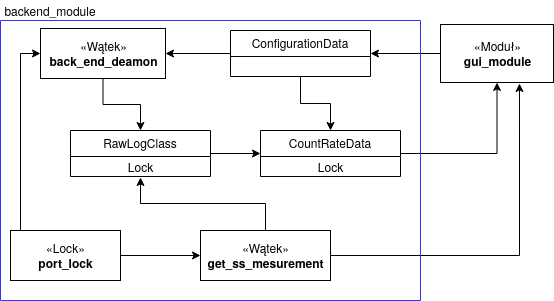
\includegraphics[width=0.65\textwidth]{Schemat_zapotrzebowania.png}
        \caption{Schemat zapotrzebowania na zasoby przez elementy programu}
        \label{program zapotrzebowanie}
\end{figure}

Klasa \textit{CountRateData} oprócz przetrzymywania danych o zliczeniach dla każdego kanału również zawiera informacje o czasie akwizycji, dzięki temu możliwe jest przekazywanie informacji do wizualizacji już jako częstotliwości zliczeń. 

Dodatkową funkcjonalnością programu jest możliwość przeprowadzenia pojedynczego badania nazywanego \textit{Single Shoot} lub skrótowo \textit{ss}.
Funkcja ta pozwala na wizualizację w postaci wykresu słupkowego pojedynczego badania w przeciwieństwie do domyślnego układu wizualizacji który jest stale aktualizowany. 
W celu przeprowadzenia takiego pomiaru wątek \textit{get\_ss\_mesurements} zamyka mutexy odpowiedzialne za port seryjny oraz Klasę logu. 
Tym sposobem wstrzymywane są inne funkcje programu aż do zakończenia pomiaru \textit{Single Shoot}.
Pomiar kończy się komendą wstrzymania pracy licznika pozwalając na zmianę konfiguracji przed kolejnymi pomiarami.  

Dane pomiarowe są zapisywane w chwili gdy: Program zostanie zamknięty, wciśnięty zostanie guzik \textit{force save}, lub minie czas auto zapisu ustawiany w interfejsie użytkownika. 

Przed zapisem tworzony zostaje folder z aktualną datą, w formacie DD-MM-YYYY, w wybranej przez użytkownika ścieżce. Nazwa pliku to godzina zapisu pliku w formacie HH:MM
Pliki są zapisywane w ustalonym formacie: JSON lub CSV.

Archiwizacja danych z akwizycji \textit{Single Shoot} jest przeprowadzana zaraz po zakończeniu pomiaru w osobnym folderze zgodnie z wcześniej przedstawioną zasadą. 

\paragraph{Fasada}
\begin{figure}
        \begin{multicols}{2}
        
        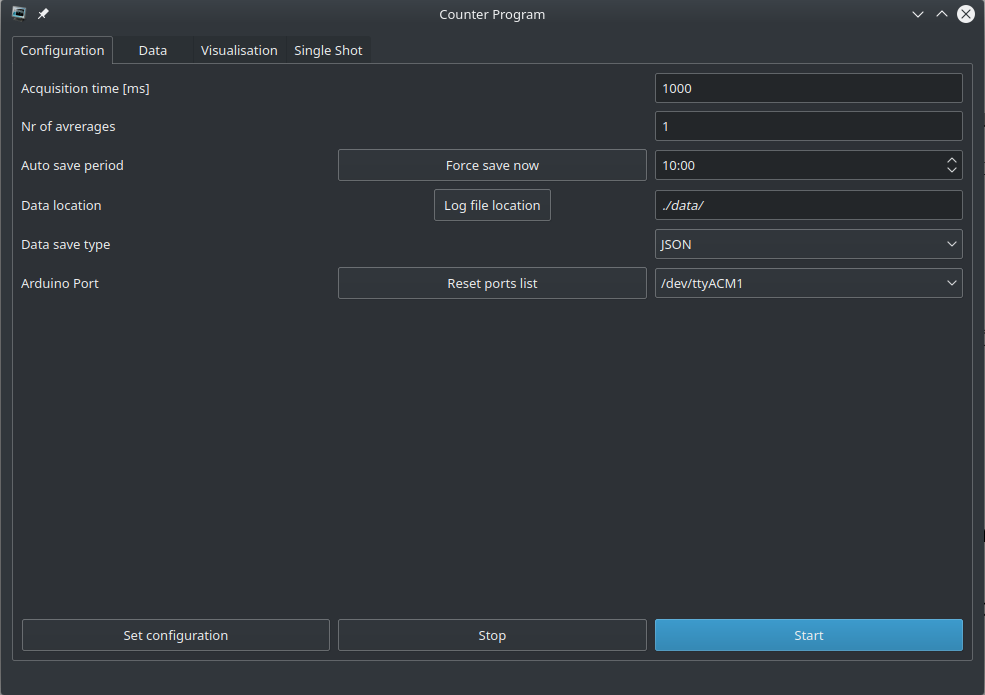
\includegraphics[width=0.49\textwidth]{configuration.png}\par
        
        
        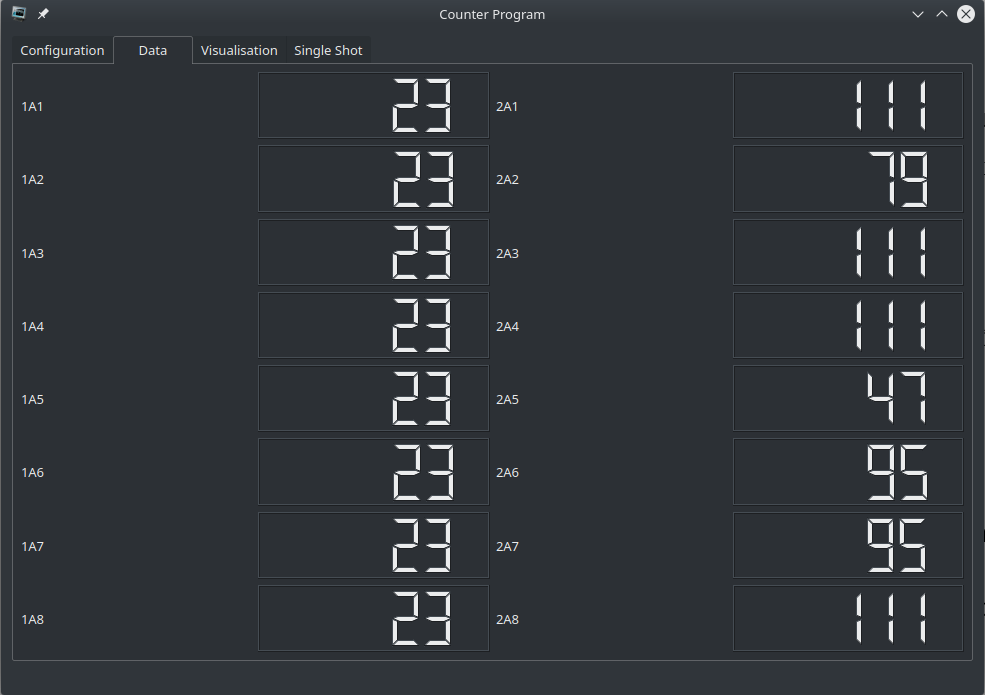
\includegraphics[width=0.49\textwidth]{digits.png}\par
        
        
        \end{multicols}\hfill
        
        \begin{multicols}{2}
        
        
        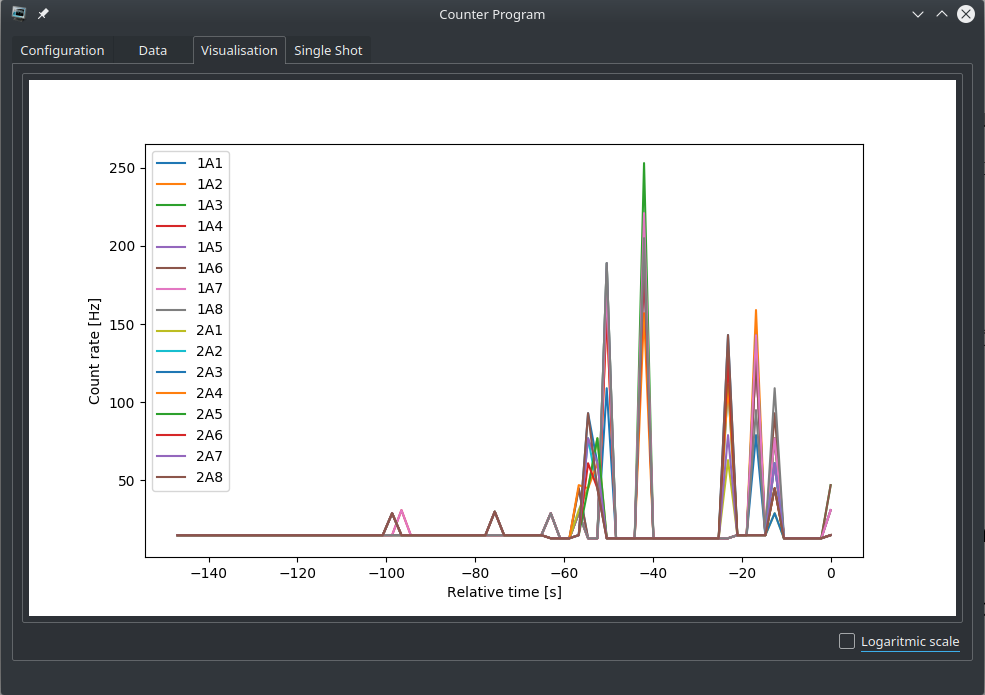
\includegraphics[width=0.49\textwidth]{wizualization.png}\par
        
        
        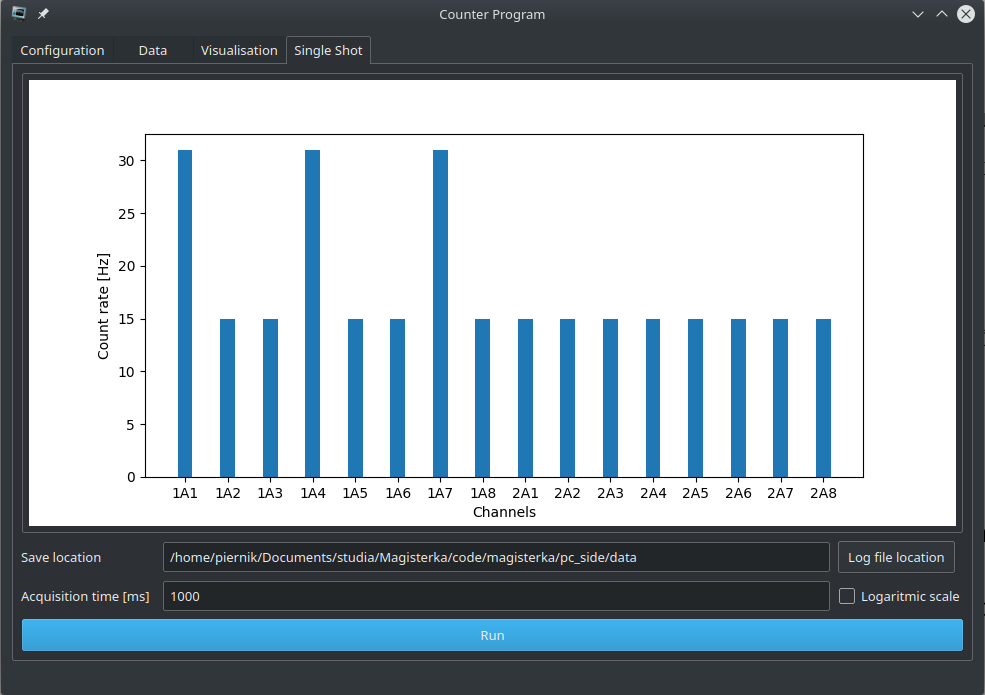
\includegraphics[width=0.49\textwidth]{wiz_ss.png}\par
        
        \end{multicols}
        \caption{Wygląd interfejsu użytkownika (linux)}
        \label{Gui pic}
        \end{figure}

Gotowy interfejs graficzny widoczny jest na rysunku \ref{Gui pic}. Jest on podzielony na cztery zakładki:
\begin{itemize}
        \item Configuration - miejsce pozwalające na rozpoczęcie pracy licznika, zatrzymanie i wszelką konfigurację dotyczącą pracy programu. 
        \item Data - prezentacja danych w postaci liczbowej 
        \item Visualization - prezentacja danych w relatywnej dziedzinie czasu. 
        \item Single Shot - Zakładka odpowiedzialna za przeprowadzenie pojedynczego badania.
\end{itemize}

Za interfejs użytkownika odpowiedzialny jest główny wątek programu, instancje klasy QTimer\cite{doc pyqt} generują one sygnały aktualizujące dane licznika oraz stgnały aktualizacji wykresu zliczeń. 
Do generowania grafik zastosowana została biblioteka matplotlib\cite{doc matplotlib}. 

Przy wykresach znajduje się pole które po odznaczeniu pozwala na wizualizację danych w logarytmicznej sali częstotliwości zliczeń.
